\chapter{Обзор}
\label{ch:view}

    Актуальность темы данной работы связана с распознаванием пожаров в реальном времени с помощью портативного вычислителя на беспилотнике. Это важная и актуальная задача, поскольку по данным МЧС, в течение 2023 года пожарно-спасательные подразделения реагировали на более чем 350 тыс. пожаров, в которых погибло порядка 7,2 тыс. человек. Количество травмированных на пожарах в 2023 г. по сравнению с 2022 г. незначительно уменьшилось – на 0,18\% (в 2022 г. – 8 521 чел.) Материальный ущерб, причиненный пожарами в 2023 г., по сравнению с 2022 г. вырос на 9,57\% (в 2022 г. – 19 774 759 тыс. руб.) по данным, приведённым на \hyperref[fig:fire_damage]{Рисунке 1}.

    \begin{figure}[ht]
        \centering
        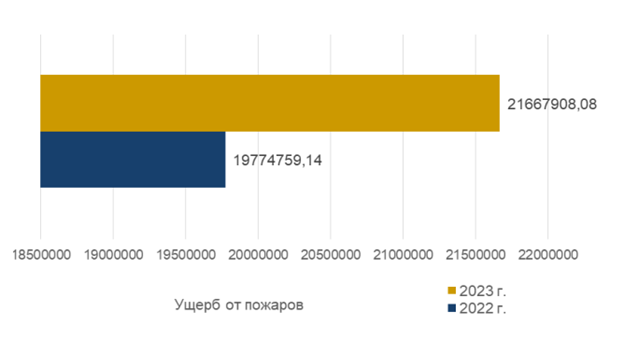
\includegraphics[width=0.7\textwidth]{fire_damage}
        \caption{Ущерб от пожаров}
        \label{fig:fire_damage}
    \end{figure}

    На территории России ежегодно регистрируется от 10 до 35 тыс. лесных пожаров, охватывающих площади от 0,5 до 2,5 млн. га. С учетом горимости лесов на неохраняемых и эпизодически охраняемых территориях севера Сибири и Дальнего Востока общая площадь, пройденная огнем, составляет от 2 до 5,5 млн. га. В нашей стране от 80 до 93\% всех пожаров в зависимости от региона возникает в 10-ки­лометровой зоне вокруг городов и поселков, вероятно, причины возникновения этих пожаров — антропогенные — вызваны людьми.

    Пожары оказывают воздействия на все компоненты экосистемы, которые проявляются в изменении разнообразия, продуктивности и функциональной структуре биоценозов.

    Естественные пожары (вызванные молниями), отличаются от антропогенных (вызванных людьми). Так, молнии, как правило, попадают в деревья на возвышенностях, и огонь, спускаясь по склону, продвигается медленно. При этом теряется сила пламени, и огонь редко распространяется на большие площади. Антропогенные же пожары чаще начинаются в низинах и распадках, что определяет более быстрое и опасное развитие.

    Естественные лесные пожары обычно оказывают положительное влияние на состояние лесов, антропогенные же – разрушительное и вредное воздействие, которое люди стараются компенсировать организацией противопожарной защиты и оперативным тушением возгораний.

    Естественные лесные пожары являются исторически постоянным фактором формирования лесов северного полушария, определяющим состояние и динамику лесного фонда. Пожары играют важную роль в формировании ландшафтов, обеспечивают периодическую смену хвойных и лиственных пород, полезную для леса, являются действенным профилактическим средством против более сильных пожаров. Средняя частота лесных пожаров в неосвоенных лесах колеблется от 50 до 100 лет, такая периодичность естественна и даже благоприятна для леса.
    
    При пожарах происходит образование большого количества окислов углерода и азота, а также золы, содержащей легкорастворимые соединения, снижается кислотность почвы, стабилизируется режим увлажнения субстрата, улучшается теплообеспеченность минеральных горизонтов почвы, ускоряется разложение органического вещества и улучшаются условия минерального питания растений.
    
    Снижается конкуренция со стороны нижних ярусов растительности, уменьшается количество мышевидных грызунов, полностью раскрываются шишки прошлых лет, высвобождая сохраняющийся в них запас семян. Все это на фоне отсутствия конкуренции за свет и влагу становится основой быстрого восстановления растительности на гарях.
    
    Среди древесных пород многие занимают значительные площади в лесах только благодаря пожарам — сосна, лиственница, береза и осина. У сосны и лиственницы выработались приспособительные особенности — толстая кора в нижней части стволов, глубокая корневая система, высоко поднятая крона. Кроме того, слой опавшей лиственничной хвои, благодаря ее особой структуре, практически не горит, поэтому густые куртины из молодых лиственниц пожар обходит стороной. Береза, будучи повреждена пожаром, дает обильную пневую поросль, а осина еще более обильную поросль от корней. У некоторых американских сосен шишки раскрываются только после пожара, когда на оголенной пожаром почве создается благоприятная среда для прорастания семян. В тропических лесах Индии встречаются древесные породы, устойчивые к огню даже в стадии подроста.

    Антропогенные пожары отличаются от естественных в первую очередь частотой. Когда пожары происходят раз в 20–30 лет или чаще, леса не успевают полноценно восстанавливаться. Таким образом частые пожары, происходящие по вине человека, ведут к уничтожению лесов. Территории видоизменяются – превращаются в пустыри, луга, болота, заросли кустарников. 

    Второе отличие антропогенных пожаров от естественных – неравномерное распределение по территории. Более 90\% пожаров происходят в радиусе 10 км вокруг населенных пунктов, в результате частота пожаров на одних и тех же местах превышает естественную в разы и десятки раз.

    Еще одна особенность лесных пожаров – преобладание сильных пожаров. В естественных условиях чаще всего возникают слабые и средние пожары, которые являются своего рода профилактикой сильных пожаров. Вблизи населенных пунктов, где леса охраняются, слабые и средние пожары быстро тушат, в результате в лесах накапливается много горючих материалов. При возникновении в таком лесу пожара, особенно в условиях засухи, он часто приобретает такую силу, что выходит из-под контроля людей и распространяется на очень большой площади.

    Таким образом, проблема пожаров является актуальной и требует эффективных решений для обеспечения безопасности населения и окружающей среды. Одним из перспективных направлений является использование беспилотных летательных аппаратов (БПЛА) для обнаружения и тушения пожаров в труднодоступных и опасных местах.

    Беспилотный летательный аппарат (БПЛА) — воздушное судно без экипажа на его борту. БПЛА могут обладать разной степенью автономности — от управляемых дистанционно до полностью автоматических, а также различаются по конструкции, назначению и другим параметрам. Управление БПЛА может осуществляться эпизодической подачей команд или непрерывно, в последнем случае БПЛА называют дистанционно-пилотируемым летательным аппаратом (ДПЛА). БПЛА применяются для решения широкого спектра гражданских и военных задач (мониторинг, съёмка и картографирование местности в научных или иных целях, доставка почты и других грузов, оказание помощи в чрезвычайных ситуациях) в разных секторах экономики (сельском хозяйстве, строительстве, энергетике). Основным преимуществом БПЛА является существенно меньшая стоимость их создания и эксплуатации (при условии сопоставимой эффективности выполнения поставленных задач). Важным фактором является то, что оператор боевого БПЛА не рискует своей жизнью, в отличие от пилота боевого самолёта. Недостатком БПЛА является уязвимость систем дистанционного управления, что особенно важно для БПЛА военного назначения. 

    Также БПЛА могут использоваться для мониторинга и обнаружения чрезвычайных ситуаций, в том числе и пожаров \hyperref[fig:EMERCOM_drone]{(см. Рисунок 2)}. Именно поэтому Министерство Российской Федерации по делам гражданской обороны, чрезвычайным ситуациям и ликвидации последствий стихийных бедствий активно использует их в своей работе. В настоящее время в системе МЧС России на оснащении реагирующих подразделений находится 1591 единица беспилотных авиационных систем, в том числе:

    \begin{itemize}
        \item 1554 единицы вертолетного (мультироторного) типа, из них 132 единицы оснащены тепловизорами;
        \item 37 единиц самолетного типа.
    \end{itemize}

    \begin{figure}[ht]
        \centering
        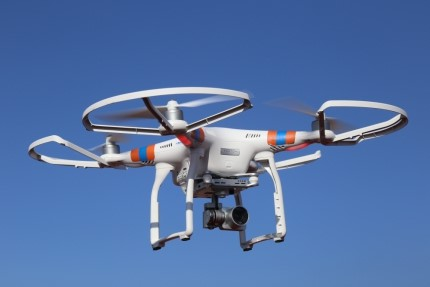
\includegraphics[width=0.5\textwidth]{EMERCOM_drone}
        \caption{Беспилотник МЧС}
        \label{fig:EMERCOM_drone}
    \end{figure}

    В 2017 году организовано и осуществлено свыше 17 000 полетов БАС, в том числе более 3 500 полетов при реагировании на ЧС. Всего налет составил свыше 2 800 часов. В ходе осуществления воздушного патрулирования мониторинга пожароопасной, паводковой и ледовой обстановки, а также, в 2017 году обследована территория площадью более 13 500 км2.

    Таким образом, распознавание пожаров в реальном времени с помощью портативного вычислителя на беспилотном летательном аппарате является актуальной и важной задачей, которая может помочь в автономном режиме отслеживать возгорания и оперативно об этом сообщать, что поможет в значительной степени снизить материальный ущерб, причиненный пожарами.

    Основная идея данного решения заключается в использовании нейросетевых технологий для детекции пожаров на видео с беспилотника. Нейронные сети — это математические модели, построенные по принципу организации биологических нейронных сетей, то есть сетей нервных клеток живого организма. Они представляют собой систему соединённых и взаимодействующих между собой простых процессоров (искусственных нейронов), способных выполнять сложные задачи благодаря своему взаимодействию. Нейронные сети используются в различных областях, таких как распознавание образов, прогнозирование, управление и другие. Нейронные сети являются мощным инструментом для анализа и обработки изображений, позволяя выявлять и классифицировать объекты на них. Применительно к задаче распознавания пожаров, нейронные сети могут быть использованы для автоматического обнаружения очагов возгорания, определения их местоположения и интенсивности, а также для оценки степени опасности пожара.

    Но перед тем, как использовать конкретную нейронную сеть необходимо понять: что такое нейронные сети и как они обучаются, какие они бывают и в чем их отличия, какая нейронка наилучшим образом подходит для реализации нашего проекта?

    Нейронная сеть — это последовательность нейронов, соединенных между собой синапсами. Структура нейронной сети пришла в мир программирования прямиком из биологии. Благодаря такой структуре машина обретает способность анализировать и даже запоминать различную информацию. Нейронные сети также способны не только анализировать входящую информацию, но и воспроизводить ее из своей памяти. Другими словами, нейросеть это машинная интерпретация мозга человека, в котором находятся миллионы нейронов, передающих информацию в виде электрических импульсов. Искусственный нейрон, из которых состоит нейронная сеть, имеет намного более простую структуру: у него есть несколько входов, на которых он принимает различные сигналы, преобразует их и передает другим нейронам. Другими словами, искусственный нейрон — это такая функция $R^n\rightarrow R$, которая преобразует несколько входных параметров в один выходной.

    Как видно на \hyperref[fig:artificial_neuron_diagram]{Рисунке 3}, у нейрона есть $n$ входов $x_i$, у каждого из которого есть вес $w_i$, на который умножается сигнал, проходящий по связи. После этого взвешенные сигналы $x_i\bullet w_i$ направляются в сумматор, который аггрегирует все сигналы во взвешенную сумму. Эту сумму также называют $net$. Таким образом, $net\ =\ \sum_{i=1}^{i=n}w_i\bullet x_i\ =\ w^T\bullet x$.

     \begin{figure}[ht]
        \centering
        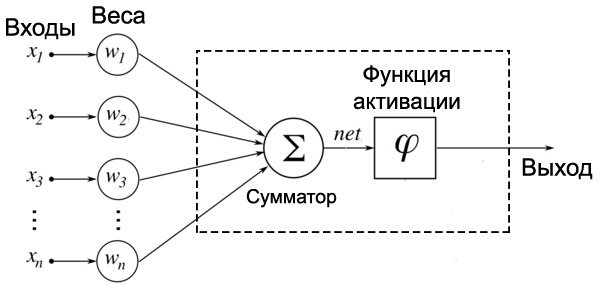
\includegraphics[width=0.7\textwidth]{artificial_neuron_diagram}
        \caption{Схема искусственного нейрона}
        \label{fig:artificial_neuron_diagram}
    \end{figure}

    Просто так передавать взвешенную сумму $net$ на выход достаточно бессмысленно — нейрон должен ее как-то обработать и сформировать адекватный выходной сигнал. Для этих целей используют функцию активации, которая преобразует взвешенную сумму в какое-то число, которое и будет являться выходом нейрона. Функция активации обозначается $\phi(net)$. Таким образом, выходов искусственного нейрона является $\phi(net)$. Для разных типов нейронов используют самые разные функции активации, но одними из самых популярных являются:

    \begin{itemize}
        \item \textbf{Функция единичного скачка}.
            Если $net > threshold$, $\phi(net) = 1$, а иначе $0$;
        \item \textbf{Сигмоидальная функция}.
            $\phi(net) = \frac{1}{1\ +\ exp(-a\bullet n e t)}$, где параметр $a$, характеризует степень крутизны функции;
        \item \textbf{Гиперболический тангенс}.
            $\phi(net) = tanh(\frac{net}{a})$, где параметр a также определяет степень крутизны графика функции;
        \item \textbf{Rectified linear units (ReLU)}.
            $
                ReLU(x) =
                \begin{cases}
                    x, x \geq 0 \\
                    x < 0 = maxx, 0
                \end{cases}
            $
    \end{itemize}
    
    Разобравшись с тем, как устроен нейрон в нейронной сети, осталось понять, как их в этой сети располагать и соединять. Как правило, в большинстве нейронных сетей есть так называемый входной слой, который выполняет только одну задачу — распределение входных сигналов остальным нейронам. Нейроны этого слоя не производят никаких вычислений. В остальном нейронные сети делятся на основные категории:

    \textbf{Однослойная нейронная сеть} (англ. Single-layer neural network) — сеть, в которой сигналы от входного слоя сразу подаются на выходной слой, который и преобразует сигнал и сразу же выдает ответ.

    Как видно из \hyperref[fig:single-layer_neural_network_scheme]{Рисунка 4} однослойной нейронной сети , сигналы $x_1,x_2,\cdots,x_n$ поступают на входной слой (который не считается за слой нейронной сети), а затем сигналы распределяются на выходной слой обычных нейронов. На каждом ребре от нейрона входного слоя к нейрону выходного слоя написано число — вес соответствующей связи.

     \begin{figure}[ht]
        \centering
        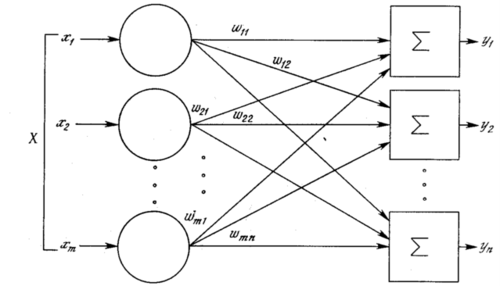
\includegraphics[width=0.7\textwidth]{single-layer_neural_network_scheme}
        \caption{Схема однослойной нейронной сети}
        \label{fig:single-layer_neural_network_scheme}
    \end{figure}

    \textbf{Многослойная нейронная сеть} (англ. Multilayer neural network) — нейронная сеть, состоящая из входного, выходного и расположенного(ых) между ними одного (нескольких) скрытых слоев нейронов \hyperref[fig:multilaye_neural_network_scheme]{(см. Рисунок 5}. Помимо входного и выходного слоев эти нейронные сети содержат промежуточные, скрытые слои. Такие сети обладают гораздо большими возможностями, чем однослойные нейронные сети, однако методы обучения нейронов скрытого слоя были разработаны относительно недавно.
	
    \begin{figure}[ht]
        \centering
        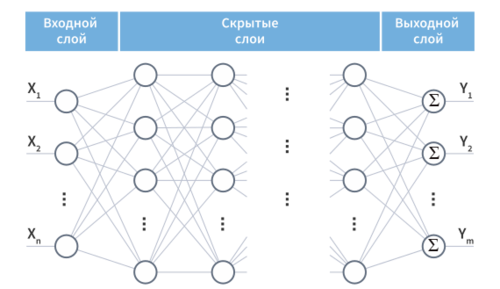
\includegraphics[width=0.7\textwidth]{multilaye_neural_network_scheme}
        \caption{Схема многослойной нейронной сети}
        \label{fig:multilaye_neural_network_scheme}
    \end{figure}

    \textbf{Сети прямого распространения} (англ. Feedforward neural network) (feedforward сети) — искусственные нейронные сети, в которых сигнал распространяется строго от входного слоя к выходному. В обратном направлении сигнал не распространяется. Все сети, описанные выше, являлись сетями прямого распространения, как следует из определения. Такие сети широко используются и вполне успешно решают определенный класс задач: прогнозирование, кластеризация и распознавание.

    \textbf{Сети с обратными связями} (англ. Recurrent neural network) — искусственные нейронные сети, в которых выход нейрона может вновь подаваться на его вход. В более общем случае это означает возможность распространения сигнала от выходов к входам. В сетях прямого распространения выход сети определяется входным сигналом и весовыми коэффициентами при искусственных нейронах. В сетях с обратными связями выходы нейронов могут возвращаться на входы. Это означает, что выход какого-нибудь нейрона определяется не только его весами и входным сигналом, но еще и предыдущими выходами.

    Обучение нейронной сети — поиск такого набора весовых коэффициентов, при котором входной сигнал после прохода по сети преобразуется в нужный нам выходной. Это определение «обучения нейронной сети» соответствует и биологическим нейросетям. Наш мозг состоит из огромного количества связанных друг с другом нейросетей, каждая из которых в отдельности состоит из нейронов одного типа (с одинаковой функцией активации). Наш мозг обучается благодаря изменению синапсов — элементов, которые усиливают или ослабляют входной сигнал. Если обучать сеть, используя только один входной сигнал, то сеть просто «запомнит правильный ответ», а как только мы подадим немного измененный сигнал, вместо правильного ответа получим бессмыслицу. Мы ждем от сети способности обобщать какие-то признаки и решать задачу на различных входных данных. Именно с этой целью и создаются обучающие выборки.

    Обучающая выборка — конечный набор входных сигналов (иногда вместе с правильными выходными сигналами), по которым происходит обучение сети. После обучения сети, то есть, когда сеть выдает корректные результаты для всех входных сигналов из обучающей выборки, ее можно использовать на практике. Однако прежде, чем сразу использовать нейронную сеть, обычно производят оценку качества ее работы на так называемой тестовой выборке. Тестовая выборка — конечный набор входных сигналов (иногда вместе с правильными выходными сигналами), по которым происходит оценка качества работы сети. Само обучение нейронной сети можно разделить на два подхода: обучение с учителем и обучение без учителя. В первом случае веса меняются так, чтобы ответы сети минимально отличались от уже готовых правильных ответов, а во втором случае сеть самостоятельно классифицирует входные сигналы.

    Исходя из поставленных целей и задач проекта, для достижения результата нам потребуется технология компьютерного зрения. Компьютерное зрение — это научное направление в области искусственного интеллекта и связанные с ним технологии получения изображений объектов реального мира, их обработки и использования полученных данных для решения разного рода прикладных задач без участия (полного или частичного) человека. Все задачи компьютерного зрения сводятся к анализу изображения или видеопотока (по сути, представляющего из себя набор сменяющихся изображений), на котором требуется прежде всего выделить фрагмент, содержащий необходимую информацию. Для выделения обычно используют или прямоугольную область, которая ограничивает исходный фрагмент, или просто выделяют пиксели, принадлежащие ему.

    Задачи компьютерного зрения:
    \begin{itemize}
        \item Идентификация. \\
            Задача идентификации состоит в том, чтобы классифицировать изображение целиком. Для этого на изображении выделяются ключевые области и по ним происходит классификация, например с помощью решающих деревьев, или сверточных нейронных сетей.
        \item Распознавание объектов. \\
            Задача состоит в том, чтобы по изображению суметь выделить на нем некоторый набор объектов. Пока задача не решена в общем случае – алгоритм не может классифицировать случайные объекты на изображении. Однако способен распознавать заранее заученный набор объектов с достаточно высокой точностью. Самым простым методом детекции объектов является метод скользящего окна методом R-CNN(англ. Regions with Convulational Neural Network - Выделение регионов с помощью свертоных сетей), при котором мы проходимся некоторым окном фиксированного размера по каждому кусочку картинки, и применяем к нему простой классификатор, обученный распознавать заранее определенный набор объектов.
        \item Сегментация изображений. \\
            Задача похожая на детекцию объектов, но в отличие от нее требуется не окружить найденные объекты рамками, а выделить пиксели, которые этот объект составляют. Сегментация применяется во многих областях, например, в производстве для индикации дефектов при сборке деталей, в медицине для первичной обработки снимков, также для составления карт местности по снимкам со спутников.
        \item Оценка положения, \\
            Задача оценки положения объекта(англ. Pose Estimation), в некотором роде продолжающая задачу сегментации. Заключается в выделении некоторого каркаса объекта (например скелета, если речь идет о людях) и определении положения этого каркаса на изображении. Этот скелет может быть использован в последствии например для предсказания направления движения. В зависимости от количества рассматриваемых объектов различают одиночную оценку положения(англ. Single-person pose estimation) и множественную(англ. Multi-person pose estimation). Различие состоит в том, что во втором случае необходимо также учитывать, что объекты могут накладываться друг на друга.
        \item Распознавание текста. \\
            Одна из ключевых задач компьютерного зрения. Сначала с помощью алгоритмов детекции выделяется область в которой текст написан, затем производится непосредственно распознавание текста например с помощью алгоритмов сегментации. При этом задачи распознавания текста написанного на листе бумаги, и распознавания текста написанного где-то на изображении, например текст на дорожном знаке, номер машины и т. д., сильно различаются, в силу наличия в последнем случае помех, которые мешают выделить конкретные буквы. В этом случае может помочь, например обучение предсказания буквы по остальным буквам в слове.
        \item Анализ видео. \\
            Так как видео представляет из себя набор изображений, одинакового размера, обычно сделанных через разные интервалы времени, то для него применимы все те задачи, которые были описаны ранее. Также появляются такие задачи как предсказание движения, заключающееся в том, чтобы по набору кадров предсказать положение объекта в следующих кадрах, или более общая задача ситуационный осведомленности(англ. Situation Awarness), заключающаяся в том, чтобы для каждого объекта в видео уметь определить его положение и статус на всех кадрах видео.
    \end{itemize}

    Важную роль в компьютерном зрении играют сверточные нейронные сети (CNN). Свёрточная нейронная сеть (англ. convolutional neural network, CNN) — специальная архитектура искусственных нейронных сетей, нацеленная на эффективное распознавание образов, входит в состав технологий глубокого обучения. Использует некоторые особенности зрительной коры, в которой были открыты так называемые простые клетки, реагирующие на прямые линии под разными углами, и сложные клетки, реакция которых связана с активацией определённого набора простых клеток. Таким образом, идея свёрточных нейронных сетей заключается в чередовании свёрточных слоёв и субдискретизирующих слоёв. Структура сети — однонаправленная (без обратных связей), принципиально многослойная. Для обучения используются стандартные методы, чаще всего метод обратного распространения ошибки. Функция активации нейронов (передаточная функция) — любая, по выбору исследователя. Название архитектура сети получила из-за наличия операции свёртки, суть которой в том, что каждый фрагмент изображения умножается на матрицу (ядро) свёртки поэлементно, а результат суммируется и записывается в аналогичную позицию выходного изображения.

    Таким образом, для нашего проекта наиболее подходит задача распознавания объектов на видео.

    Следующим этапом является выбор технологического стека для реализации и разработки нашего проекта. В первую очередь это выбор языка программирования – это важнейшее решение, от которого во многом зависит успех всей разработки. Анализ всех факторов, понимание требований проекта и готовность к изменениям — это залог правильного выбора языка, который позволит реализовать наш проект наиболее эффективным и успешным образом. Существует множество аспектов, которые необходимо учитывать при выборе языка программирования. Первым компонентом является сама задача, которую предстоит решить. Каждый язык программирования имеет свои сильные стороны и области применения.  В нашем случае отлично подходит язык программирования Python, который хорошо зарекомендовал себя для задач связанных с анализом данных и машинным обучением. По сути, машинное обучение — это технология, которая помогает приложениям на основе искусственного интеллекта обучаться и выдавать результаты автоматически, без человеческого вмешательства. В чем состоит работа специалиста по машинному обучению? Он должен собирать, систематизировать и анализировать данные, а затем на основе полученной информации создавать алгоритмы для искусственного интеллекта. Python лучше всего подходит для выполнения таких задач, потому что он довольно понятный по сравнению с другими языками. Более того, у него отличная производительность при обработке данных. Одна из основных причин, почему Python используется для машинного обучения состоит в том, что у него есть множество фреймворков, которые упрощают процесс написания кода и сокращают время на разработку. В научных расчетах используется Numpy, в продвинутых вычислениях — SciPy, в извлечении и анализе данных — SciKit-Learn. Эти библиотеки работают в таких фреймворках, как TensorFlow, CNTK и Apache Spark. Существует фреймворк для Python, разработанный специально для машинного обучения — это PyTorch. Python — самый высокоуровневый и понятный язык, с которым удобно работать. Благодаря его лаконичности и удобству чтения он хорошо подходит для обучения разработке ПО. Кроме того, Python хорошо подходит для машинного обучения, потому что сами алгоритмы машинного обучения сложны для понимания. При работе с Python разработчику не нужно уделять много внимания непосредственно написанию кода: все внимание он может сосредоточить на решении более сложных задач, связанных с машинным обучением. Простой синтаксис языка Python помогает разработчику тестировать сложные алгоритмы с минимальной тратой времени на их реализацию. Еще одно преимущество Python — это обширная поддержка и качественная документация. Существует множество полезных ресурсов о Python, на которых программист может получить помощь и консультацию, находясь на любом этапе разработки. Следующее преимущество Python в машинном обучении состоит в его гибкости: например, у разработчика есть выбор между объектно-ориентированным подходом и скриптами. Python помогает объединять различные типы данных. Более того, Python особенно удобен для тех разработчиков, которые большую часть кода пишут с помощью IDE. Еще немаловажным фактором является навык работы команды разработчиков с данным языком программирования. Почти все в нашей команде ранее работали с Python. Исходя из всего вышеперечисленного, самым оптимальным языком программирования в условиях нашего проекта является Python.

    В качестве модели для обнаружения пожаров на видео было решено использовать YOLOv8. YOLOv8 - это новейшее семейство моделей обнаружения объектов на базе YOLO от Ultralytics, обеспечивающих самые современные характеристики. По сравнению с предыдущими версиями YOLO, модель YOLOv8 работает быстрее и точнее, обеспечивая при этом единую структуру для обучения моделей для выполнения обнаружение объектов, сегментация экземпляров, классификации изображений. Вот некоторые ключевые особенности новой версии:

    \begin{itemize}
        \item Удобный для пользователя API (командная строка + Python).
        \item Быстрее и точнее.
        \item Поддерживает:
            \begin{itemize}
                \item Обнаружение объектов,
                \item Сегментация экземпляров,
                \item Классификация изображений.
            \end{itemize}
        \item Расширяемый для всех предыдущих версий.
        \item Новая Backbone сеть.
        \item Новая Anchor-Free head.
        \item Новая функция потерь.
    \end{itemize}

    YOLOv8 также обладает высокой эффективностью и гибкостью, поддерживает множество форматов экспорта, и модель может работать на CPU и GPU.

    Для удобного написания кода разработчикам была нужна система, которая бы помогала им в работе с несколькими версиями приложения, поэтому ими было принято решение использовать Git. 

    Git - это распределенная система контроля версий, которая широко используется в разработке программного обеспечения. Она предоставляет разработчикам мощные инструменты для эффективного управления изменениями в исходном коде. Почему же именно Git был выбран в качестве решения этой проблемы? Ответим на этот вопрос:

    \begin{itemize}
        \item Одно из ключевых преимуществ Git заключается в его распределенной архитектуре. В отличие от централизованных систем контроля версий, каждый разработчик, работающий с Git-репозиторием, имеет полную копию истории изменений. Это повышает доступность данных и устойчивость к сбоям.
        \item Git предоставляет удобные средства для сотрудничества и совместной работы. Разработчики могут создавать ветки, выкладывать и получать изменения, отслеживать конфликты и вести обсуждения прямо в репозитории.
        \item Благодаря своей распределенной природе, Git позволяет разработчикам работать автономно, не зависимо от наличия подключения к центральному серверу. Это делает процесс разработки более гибким и эффективным.
        \item Git предоставляет мощные средства для ветвления и слияния. Разработчики могут создавать множество независимых веток, экспериментировать с изменениями, а затем легко объединять их обратно в основную ветвь. Это способствует параллельной разработке и упрощает процесс интеграции.
        \item Система контроля версий Git отличается своей производительностью. Она использует эффективные алгоритмы для хранения и обработки изменений, что позволяет быстро выполнять операции, даже в больших репозиториях.
        \item Git обладает развитой системой управления конфликтами при слиянии. Git предоставляет удобные инструменты, которые помогают разрешать противоречия между параллельно внесенными изменениями.
        \item Git также поддерживает нелинейную историю. Разработчики могут перемещаться по истории коммитов, отменять или изменять предыдущие изменения, создавая ветви и сливая их обратно. Это обеспечивает гибкость в управлении проектом.
        \item Git отличается своей безопасностью. Он использует криптографические хеши для идентификации коммитов, что помогает защитить историю изменений от несанкционированного доступа и повреждения.
        \item Git широко распространен и полностью поддерживается. Он является де-факто стандартом в индустрии разработки программного обеспечения и поддерживается большинством популярных платформ и инструментов.
        \item Система контроля версий Git отличается своим богатым набором команд и возможностей. Она позволяет выполнять самые разнообразные операции по управлению изменениями: просмотр истории, фиксация изменений, сравнение версий, ветвление и многое другое.
        \item Git обладает развитой системой настройки и конфигурирования. Он позволяет гибко адаптировать свое поведение под требования конкретного проекта или рабочей среды.
        \item Git полностью кроссплатформен. Он доступен для широкого спектра операционных систем, включая Windows, Linux и macOS, что облегчает его использование в различных средах разработки.
        \item Git интегрирован с различными онлайн-сервисами, такими как GitHub, GitLab и Bitbucket. Это позволяет организовывать эффективное сотрудничество и управление проектами.
    \end{itemize}

    Исходя из всего написанного в этом обзоре, можно сделать вывод о том, что именно те технологии, которые были выбраны нами на этапе планирования нашего приложения являются самыми оптимальными технологиями в условиях нашей команды и выбранного проекта, позволяющими  полноценно реализовать наш проект наиболее эффективным (с точки зрения архитектуры кода и его написания) и полноценным (с точки зрения поставленной перед нами задачей) образом.
\endinput